%~/Ripetere/sciripetere
\makeatletter
\let\@starttocorig\@starttoc
\makeatother
\documentclass[oneside,20pt,fleqn,extrafontsizes]{memoir}
%%% color definition names: xcolor
\usepackage[usenames,dvipsnames]{xcolor}
\definecolor{wocrit}{rgb}{0.75, 0.25, 0.0}
\definecolor{todo}{rgb}{0.75, 0.0, 0.2}
%%%%%%%%%%%% Hyperref package
\usepackage{hyperref}
\hypersetup{
    colorlinks,
    citecolor=black,
    filecolor=black,
    linkcolor=black,
    urlcolor=black
}
%%% Import other packages%
\usepackage{usepkg}
%% import moodded thing
\usepackage{mathOp}
%%%%%%%%%%%%%%%%%% refname, titletoc, titlesec setting
\def\csubtoc{1}%\startcontents[chapters]
\usepackage{titleT-ref}%toc depth
\usepackage{localF}
%%%%%%%%%%%%%%%%%%%%%%%%
%%%%%%%%%%%%%%%%%Geometry package
\usepackage{mygeometry}
%%%%%%%
\usepackage{fancypkg}%%%import fancy package with memoir correction
%%%%%%%%%%%%%%%%%% setlength
\usepackage{mylength}
\linespread{0.5}
%%%%%%% META
\title{workout physics: distinguere procedimento da conclusioni}
%%import makeidx
%\usepackage{makeidx}
%%% COUNTERS
\setsecnumdepth{subsection}
\setcounter{tocdepth}{0}       % chapter
%\settocdepth{chapter}
\regtotcounter{chapter}
\newcounter{cherrychapter}%[chapte]
\setcounter{cherrychapter}{1}
\newcounter{partworkouts}%[chapte]
\setcounter{partworkouts}{1}
%%%% import functions
\usepackage{functions}
\usepackage{sources}
%%%%%%%%%%%%%%%%%%%% MULTINDExssss (number of chapters)
%\makeindex[1]%biasmomentumoggi]%chapters
%\makeindex[2]%meditazione]
%\makeindex[3]%nitidezza]
%\makeindex[4]%teatro]
\begin{document}%BEGIN
\pagestyle{mystyle}%% mystyle defined in usepkg
\renewcommand*{\contentsname}{\label{toc}{Table of Contents}}%%\printcontents without head/hypereff
%\makeatletter
%\renewcommand*{\@tocmaketitle}{\label{toc}{Table of Contents}}
%\makeatother
\maketitle
\listoftodos
\tableofcontents%~/Ripetere/sciripetere*
%\documentclass[main.tex]{subfiles}
    \begin{filecontents}{procem.bib}
    @book{longair2010high,
    title={High energy astrophysics},
    author={Longair, Malcolm S},
    year={2010},
    publisher={Cambridge university press},
    keywords={}
    }
    @book{longair2003theoretical,
    title={Theoretical concepts in physics: an alternative view of theoretical reasoning in physics},
    author={Longair, Malcolm S},
    year={2003},
    publisher={Cambridge University Press},
    keywords={}
    }
    @article{passon2017planck,
    title={Planck’s radiation law, the light quantum, and the prehistory of indistinguishability in the teaching of quantum mechanics},
    author={Passon, Oliver and Grebe-Ellis, Johannes},
    journal={European Journal of Physics},
    volume={38},
    number={3},
    pages={035404},
    year={2017},
    publisher={IOP Publishing},
    keywords={}
    }
    \end{filecontents}
%\begin{document}
\part{Costanti astrofisiche}
    \chapter{Unit\'a di misura}
        \begin{itemize}
        \item Mass:
        \begin{align*}
        &u=\frac{1}{N_A}\si{\gr}\tag{atomic mass unit}
        \end{align*}
        \item Pressure:
        \begin{equation*}
        P=\frac{\text{Force}}{A}=\frac{F*d}{A*d}=\frac{\text{Energy}}{\text{Volume}}\tag{Pressure - energy density}
        \end{equation*}
        \item Momentum flux
        \begin{equation*}
        |v_i\rho\vec{v}|=\si{\meter\per\second}*\si{\gram\per\cube\meter}*\si{\meter\per\second}=\frac{p}{\si{\square\meter\per\second}}
        \end{equation*}
        \end{itemize}
\part{Leggi Termodinamica}
    \chapter{Ogni sistema macroscopico \'e un sistema termodinamico}
        \begin{itemize}
        \item Parametri termodinamici sono quantit\'a macroscopiche misurabili (P, V, T, H, \ldots)
        \item Uno stato termodinamico \'e specificato dai parametri; $f(P,V,T)=0$ definisce superficie in PVT e i punti soni stati di equilibrio.
        \item Equilibrio: stato non cambia nel tempo
        \item Equazione di stato \'e una relazione funzionale tra i parametri termodinamicidi un sistema all'equilibrio
        \item Una trasformazione termodinamica \'e un cambio di stato; una trasformazione da stato equilibrio \'e possibile per cambio condizioni esterne al sistema. La trasformazione \'e quasi-statica se \'e cos\'i lenta da passare da stati di equilibrio. Una trasformazione \'e reversibile se riportando indietro nel tempo la condizione esterna la trasformazione ripercorre la sua storia. Una trasformazione reversibile \'e quasi statica ma non nec. vv.
        \item Lavoro meccanico; per parametri PVT: $d\,W=Pd\,V$.
        \item Il calore \'e ci\'o che viene assorbito dal sistema se T aumenta senza che venga compiuto lavoro. $\Delta Q=C\Delta T$.
        \item Equazione di stato gas ideale: $PV=NkT$. Ogni gas se suff. diluito si comporta in modo universale.
        \end{itemize}
    \chapter{Prima legge}
        La quantit\'a $\Delta U=\Delta Q-\Delta W$ \'e la stessa per tutte le trasformazioni che vanno da stato A a stato B: $U$ \'e funzione di stato quindi $d\,U=d\,Q-Pd\,V$ \'e diff. esatto e l'integrale $\int d\,U$ non dipende dal percorso ma da estremi integrazione. Considero $U(P,V)$:
        \begin{align*}
        &dU=\PDy{P}{U}|_Vd\,P+\PDy{V}{U}|_Pd\,V\\
        &\PDof{V}[\PDy{P}{U}|_V]_P=\PDof{P}[\PDy{V}{U}|_P]_V\tag*{exact d}
        \end{align*}
        scegliendo come variabili indip. $(P,V), (P,T), (V,T)$:
        \begin{align*}
            &dQ=\PDy{P}{U}|_V+[\PDy{V}{U}|_P+P]d\,V\\
            &dQ=[\PDy{T}{U}|_P+P\PDy{T}{V}|_P]dT+[\PDy{T}{U}|_P+P\PDy{P}{V}|_T]d\,P\\
            &dQ=\PDy{T}{U}|_Vd\,T+[\PDy{V}{U}|_T+P]d\,V
        \end{align*}
    \chapter{Seconda Legge termodinamica}
        \begin{itemize}
        \item Enunciato kelvin: Non esiste trasformazione termodinamica il cui solo effetto \'e di estrarre calore da serbatoio e convertirlo interamente in calore
        \item Enunciato Clausius: Non esiste trasformazione il cui solo effetto \'e quello di trasferire calore da serbatoio pi\'u freddo a uno pi\'u caldo
        \end{itemize}
        \section{Teorema di Carnot}
        Una macchina di Carnot \'e una sostanza che subisce trasformazione ciclica reversibile descritta nel diagramma PV da ab isoterma $T_2$ durante la quale il sistema assorbe calore $Q_2$, bc adiabatica, isoterma a $T_1<T_2$ durante la quale sistema emette calore $Q_1$, da adiabatica; $W=Q_2-Q_1$, efficienza $\eta=\frac{W}{Q_2}=1-\frac{Q_1}{Q_2}$. Nessuna macchina che opera tra due temperature date \'e pi\'u efficiente della macchina di Carnot. Tutte le macchine di Carnot che operano tra due date temperature hanno medesima efficienza.
        \section{Teorema di Clausius - Entropia}
        In ogni trasformazione ciclica in cui \'e definita T $\oint \frac{d\,Q}{T}\leq0$: se reversibile vale =.
            Per una trasformazione reversibile $\int \frac{dQ}{T}$ \'e indipendente dal cammina della trasformazione ma dipende solo da stati iniziali: funzione di stato entropia $S(A)=\int_0^A \frac{d\,Q}{T}$; per una trasformazione arbitraria $\int_B^A \frac{d\,Q}{T}\leq S(B)-S(A)$, $=$ se reversibile; l'entropia di un sistema isolato non diminuisce mai.
        \begin{itemize}
        \item Espansione isoterma reversibile: pistone-molla immersi in reservoire a T - $\Delta Q=RT\ln{\frac{V_2}{V_1}}$ quindi $\Delta S_{gas}=\frac{\Delta Q}{T}$, $\Delta S_{reserv}=-\frac{\Delta Q}{T}$ e il lavore $W=\Delta Q$ \'e immagazzinata nella molla attaccato al pistone.
        \item Espansione Libera - $\Delta S=R\ln{\frac{V_2}{V_1}}$; potevamo estrarre energia espandendo il gas in maniera reversibile.
        \end{itemize}
        \section{Derivate parziali: relazione concatenamento}
        \begin{align*}
        &f(x,y,z)=0, f_x\PDy{y}{x}|_z+f_y=0\tag{y,z as indep vars - perm and mult:}\\
        &\PDy{y}{x}|_z\PDy{z}{y}|_x\PDy{x}{z}|_y=(-\frac{f_x}{f_y})(-\frac{f_y}{f_z})(-\frac{f_z}{f_x})=-1
        \end{align*}
        \section{Conseguenze seconda legge TD}
        \begin{itemize}
        \item Riscrivo prima legge TD in termini di $(T,V)$ e $(T,P)$: Equazioni $Td\,S$.
        \begin{align*}
        &d\,Q=C_Vd\,T+[\PDy{V}{U}|_T+P]d\,V=Td\,S\\
        &d\,S=\frac{C_V}{T}d\,T+\frac{1}{T}[\PDy{V}{U}|_T+P]d\,V=Td\,S\\
        &\PDof{V}|_T(\frac{C_V}{T})=\PDof{T}|_V[\frac{1}{T}\PDy{V}{U}|_T+\frac{P}{T}]\tag*{$dS$ \'e diff. esatto}\\
        &C_V=\TDy{T}{U}|_V: \PDy{V}{U}|_T=T\PDy{T}{P}|_V-P\\
        &Td\,S=C_Vd\,T+T\PDy{T}{P}|_Vd\,V\\
        &Td\,S=C_Pd\,T-T\PDy{T}{V}|_Pd\,P
        \end{align*}
        Definiamo le quantit\'a misurabili sperimentalmente:
        \begin{align*}
        &\alpha=\frac{1}{V}\PDy{T}{V}|_P\tag{coeff. espansione termica}\\
        &\kappa_T=-\frac{1}{V}\PDy{P}{V}|_T\tag{compr. isoterma}\\
        &\kappa_S=-\frac{1}{V}\PDy{P}{V}|_S\tag{compr. adiabatica}
        \end{align*}
        Riscrivo ancora la coppia di equazioni per $Td\,S$:
        \begin{align*}
        &\PDy{T}{P}|_V=-\frac{1}{\PDy{V}{T}|_P\PDy{P}{V}|_T}=\frac{\PDy{T}{V}|_P}{-\PDy{P}{V}|_T}=\frac{\alpha}{\kappa_T}\\
        &Td\,S=C_Vd\,T+\frac{\alpha T}{\kappa_T}d\,V\\
        &Td\,S=C_Pd\,T-\alpha TVd\,P
        \end{align*}
        \item $(C_P-C_V)$. Scegliendo $(P,V)$ come variabili indipendenti usando relazioni $Td\,S$:
        \begin{align*}
        &d\,T=\PDy{V}{T}|_Pd\,V+\PDy{P}{T}|_Vd\,P\\
        &[(C_P-C_V)\TDy{V}{T}|_P-T\PDy{T}{P}|_V]d\,V+[(C_P-C_V)\TDy{P}{T}|_V-T\PDy{T}{V}|_P]d\,P=0\\
        &C_P-C_V=\frac{T\PDy{T}{P}|_V}{\PDy{V}{T}|_P}=-T[\PDy{T}{V}|_P]^2\PDy{V}{P}|_T\\
        &C_P-C_V=\frac{TV\alpha^2}{\kappa_T}\\
        &\kappa_T\geq0\tag{T van Hove}
        \end{align*}
        \item $\gamma=\frac{C_P}{C_V}$.
        \begin{align*}
        &d\,S=0:\\
        &C_V=-T\PDy{T}{P}|_V\PDy{T}{V}|_S,\ C_P=T\PDy{T}{V}|_P\PDy{T}{P}|_S\\
        &\frac{C_P}{C_V}=\frac{\PDy{P}{V}|_T}{\PDy{P}{V}|_S}
        \end{align*}
        \item Espressione per calori specifici:
        \begin{equation*}
        C_V=\frac{TV\alpha^2\kappa_S}{(\kappa_T-\kappa_S)\kappa_T},\ C_P=\frac{TV\alpha^2}{\kappa_T-\kappa_S}
        \end{equation*}
        \end{itemize}
    \chapter{Potenziali termodinamici: equilibrio sistema non isolato}
        \begin{align}
        &A=U-TS\tag*{E libera di Helmholtz}\\
        &G=A+PV\tag*{E libera di Gibbs}
        \end{align}
        \section{Energia libera di Helmholts A}
            In una trasformazione isoterma l'energia libera A \'e uguale al massimo lavoro possibile compiuto dal sistema col segno cambiato.
            \begin{align*}
                &\frac{\Delta Q}{T}\leq\Delta S\\
                &W\leq-\Delta U+T\Delta S=-\Delta A\tag*{prima legge}\\
                &W=-\Delta A\tag*{reversibile}
            \end{align*}
            Per un sistema meccanicamente isolato e a T const. l'energia libera di Helmholtz non cresce mai.
            \subsection{Cilindro a T costante}
            Un pistone scorrevole divide il cilindro in $V_1,V_2$ con $P_1,P_2$: la posizione di equilibrio \'e quella che minimizza l'energia libera del sistema.
            \begin{align*}
            &0=\delta A=\PDy{V_1}{A}|_T\delta\,V_1+\PDy{V_2}{A}|_T\delta\,V_2=[\PDy{V_1}{A}|_T-\PDy{V_2}{A}|_T]\delta\,V_1\tag*{all'equilibrio}\\
            &P_1=P_2\tag*{relazioni di Maxwell}
            \end{align*}
        \section{Energia Libera di Gibbs}
            $G=A+PV$: Per un sistema a T e P costante l'energia libera di Gibbs non aumenta mai.
        \section{Relazioni di Maxwell}
            \begin{minipage}{0.39\textwidth}
            \begin{align*}
                &dA=-Pd\,V-Sd\,T\\
                &dG=-Sd\,T+Vd\,P\\
                &dH=Td\,S+Vd\,P\\
                &dU=-Pd\,V+Td\,S
            \end{align*}
            \end{minipage}
            \begin{minipage}{0.6\textwidth}
                \begin{tikzpicture}
                    \node (V) at (0,0) {V};
                    \node (A) [right=1cm of V.east] {A};
                    \node (T) [right=1cm of A.east] {T};
                    \node (G) [below=0.5cm of T.south] {G};
                    \node (P) [below=0.5cm of G.south] {P};
                    \node (H) [left=1cm of P.west] {H};
                    \node (S) [left=1cm of H.west] {S};
                    \node (U) [above=0.5cm of S.north] {U};
                    \draw[->] (P)--(V);
                    \draw[->] (S)--(T);
                \end{tikzpicture}
            \end{minipage}
    \chapter{Terza legge}
        La definizione di entropia dipende da esistenza trasformazione reversibile che connette lo stato di riferimento O allo stato A: esiste sempre se giacciono sullo stesso foglio della superficie definita da EOS (due sostanze o stati metastabili possono dare luogo a superficie con fogli disgiunti).
        \section{Terza Legge (Nerst)}
            L'entropia di un sistema allo zero assuluto \'e una costante universale (che pu\'o essere asunta pari a zero).
            \begin{itemize}
                \item La capacit\'a termica deve annullarsi a $T=0$: $S(A)=\int_0^{T_A}C_R(T)\frac{d\,T}{T}$.
                \item La curva di fusione nel diagramma T-P ha tangente 0 in $T=0$:
                    Il coeff. di espansione termica \'e nullo allo zero assoluto:
                    \begin{align*}
                        &\PDy{T}{S}|_P=\frac{C_P}{T},\ \PDy{P}{S}|_T=-\PDy{T}{V}|_P:\tag{$Td\,S$}\\
                        &\PDy{P}{C_P}|_T=-T\PtwoDy{T}{V}|_P\\
                        &V\alpha=\PDy{T}{V}|_P=-\PDy{P}{S}|_T=-\PDof{P}\int_0^TC_P \frac{d\,T}{T}\tag*{int const P}\\
                        &=-\int_0^T\PDy{P}{C_P}|_T \frac{d\,T}{T}=\PDy{T}{V}|_P-[\PDy{T}{V}|_P]_{T=0}\\
                        &\alpha=\frac{1}{V}\PDy{T}{V}|_P\xrightarrow{T\to0}0
                    \end{align*}
                    Analog. $\PDy{T}{P}|_V\xrightarrow{T\to0}0$.
            \end{itemize}
            \subsection{Irraggiungibilit\'a zero assoluto!(?)}
            \begin{align*}
                &C_P=T^x(a+bT+cT^2+\ldots),\ \PDy{P}{C_P}|_T=T^x(a'+b'T+c'T^2+\ldots):\\
                &\frac{V\alpha}{C_P}\xrightarrow{T\to0}\const>0
            \end{align*}
            Non si pu\'o raffreddare un sistema fino allo zero assoluto tramite una variazione finita dei parametri termodinamici: a $T=0$ la variazione di P per produrre variazione finita di T non \'e limitata ($dT=\frac{V\alpha}{C_P}Td\,P$).
\part{Stefan-Boltzmann law and LTE (sfondo processi astrofisici)}
    \begin{itemize}
    \item Radiative transfer equation: atomic emission, absorption and scattering.
    \item LTE
    \item Planck law
    \end{itemize}
    \chapter{Photon Gas and BlackBody Radiation}
        \section{Potere emissivo}
                Energia emessa per unit\'a di angolo solido, per unit\'a di superficie, per unit\'a di tempo fra $\nu,\nu+d\nu$: $e(\nu,T,x)$.
                \begin{figure}
                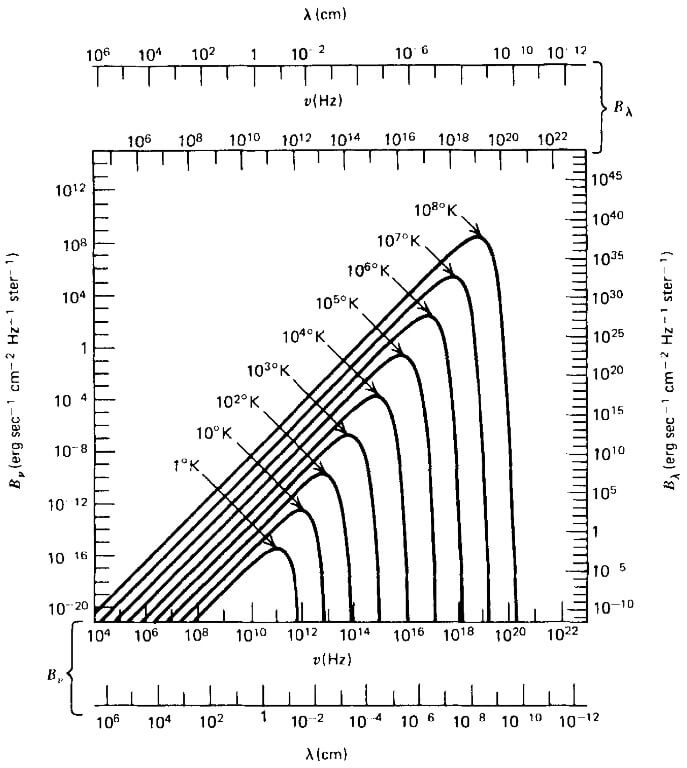
\includegraphics[trim={0cm 0cm 0 0},width=0.9\textwidth]{planckkraus}
                %\caption{}
                \label{planckkraus}
                \end{figure}
        \section{Potere Assorbente e corpo nero}
                Rapporto tra energia assorbita e energia totale: $a(\nu,T,x)$. Corpo nero ha $a=1$.
        \section{Principio di \khhff{}}
                \khhff{}(1860) ha dimostrato per via termodinamica che per un corpo in equilibrio termodinamico $\frac{e(\nu,T,x)}{a(\nu,T,x)}$ \'e indipendente da dalla natura del corpo (x): funzione universale $E(T,\nu)$. In una cavit\'a contenente corpi qualsiasi si stabilisce per mezzo di processi irreversibili uno stato stazionario della radiazione che dipende solo da T comune a tutti i corpi: lo stesso stato della radiazione nel vuoto quando le pareti della cavit\'a sono nere e hanno stessa temperatura
                \begin{align}
                    &\frac{e(\nu,T,x)}{a(\nu,T,x)}=E(\nu,T)\tag{P.di\khhff{}}\label{pkhhff}\\
                    &e=\int d\,\nu e(\ldots),\ a=\int d\,\nu a(\ldots)
                \end{align}
                \begin{itemize}
                    \item Parte 1.
                        \begin{minipage}{0.5\linewidth}
                            \centering
                            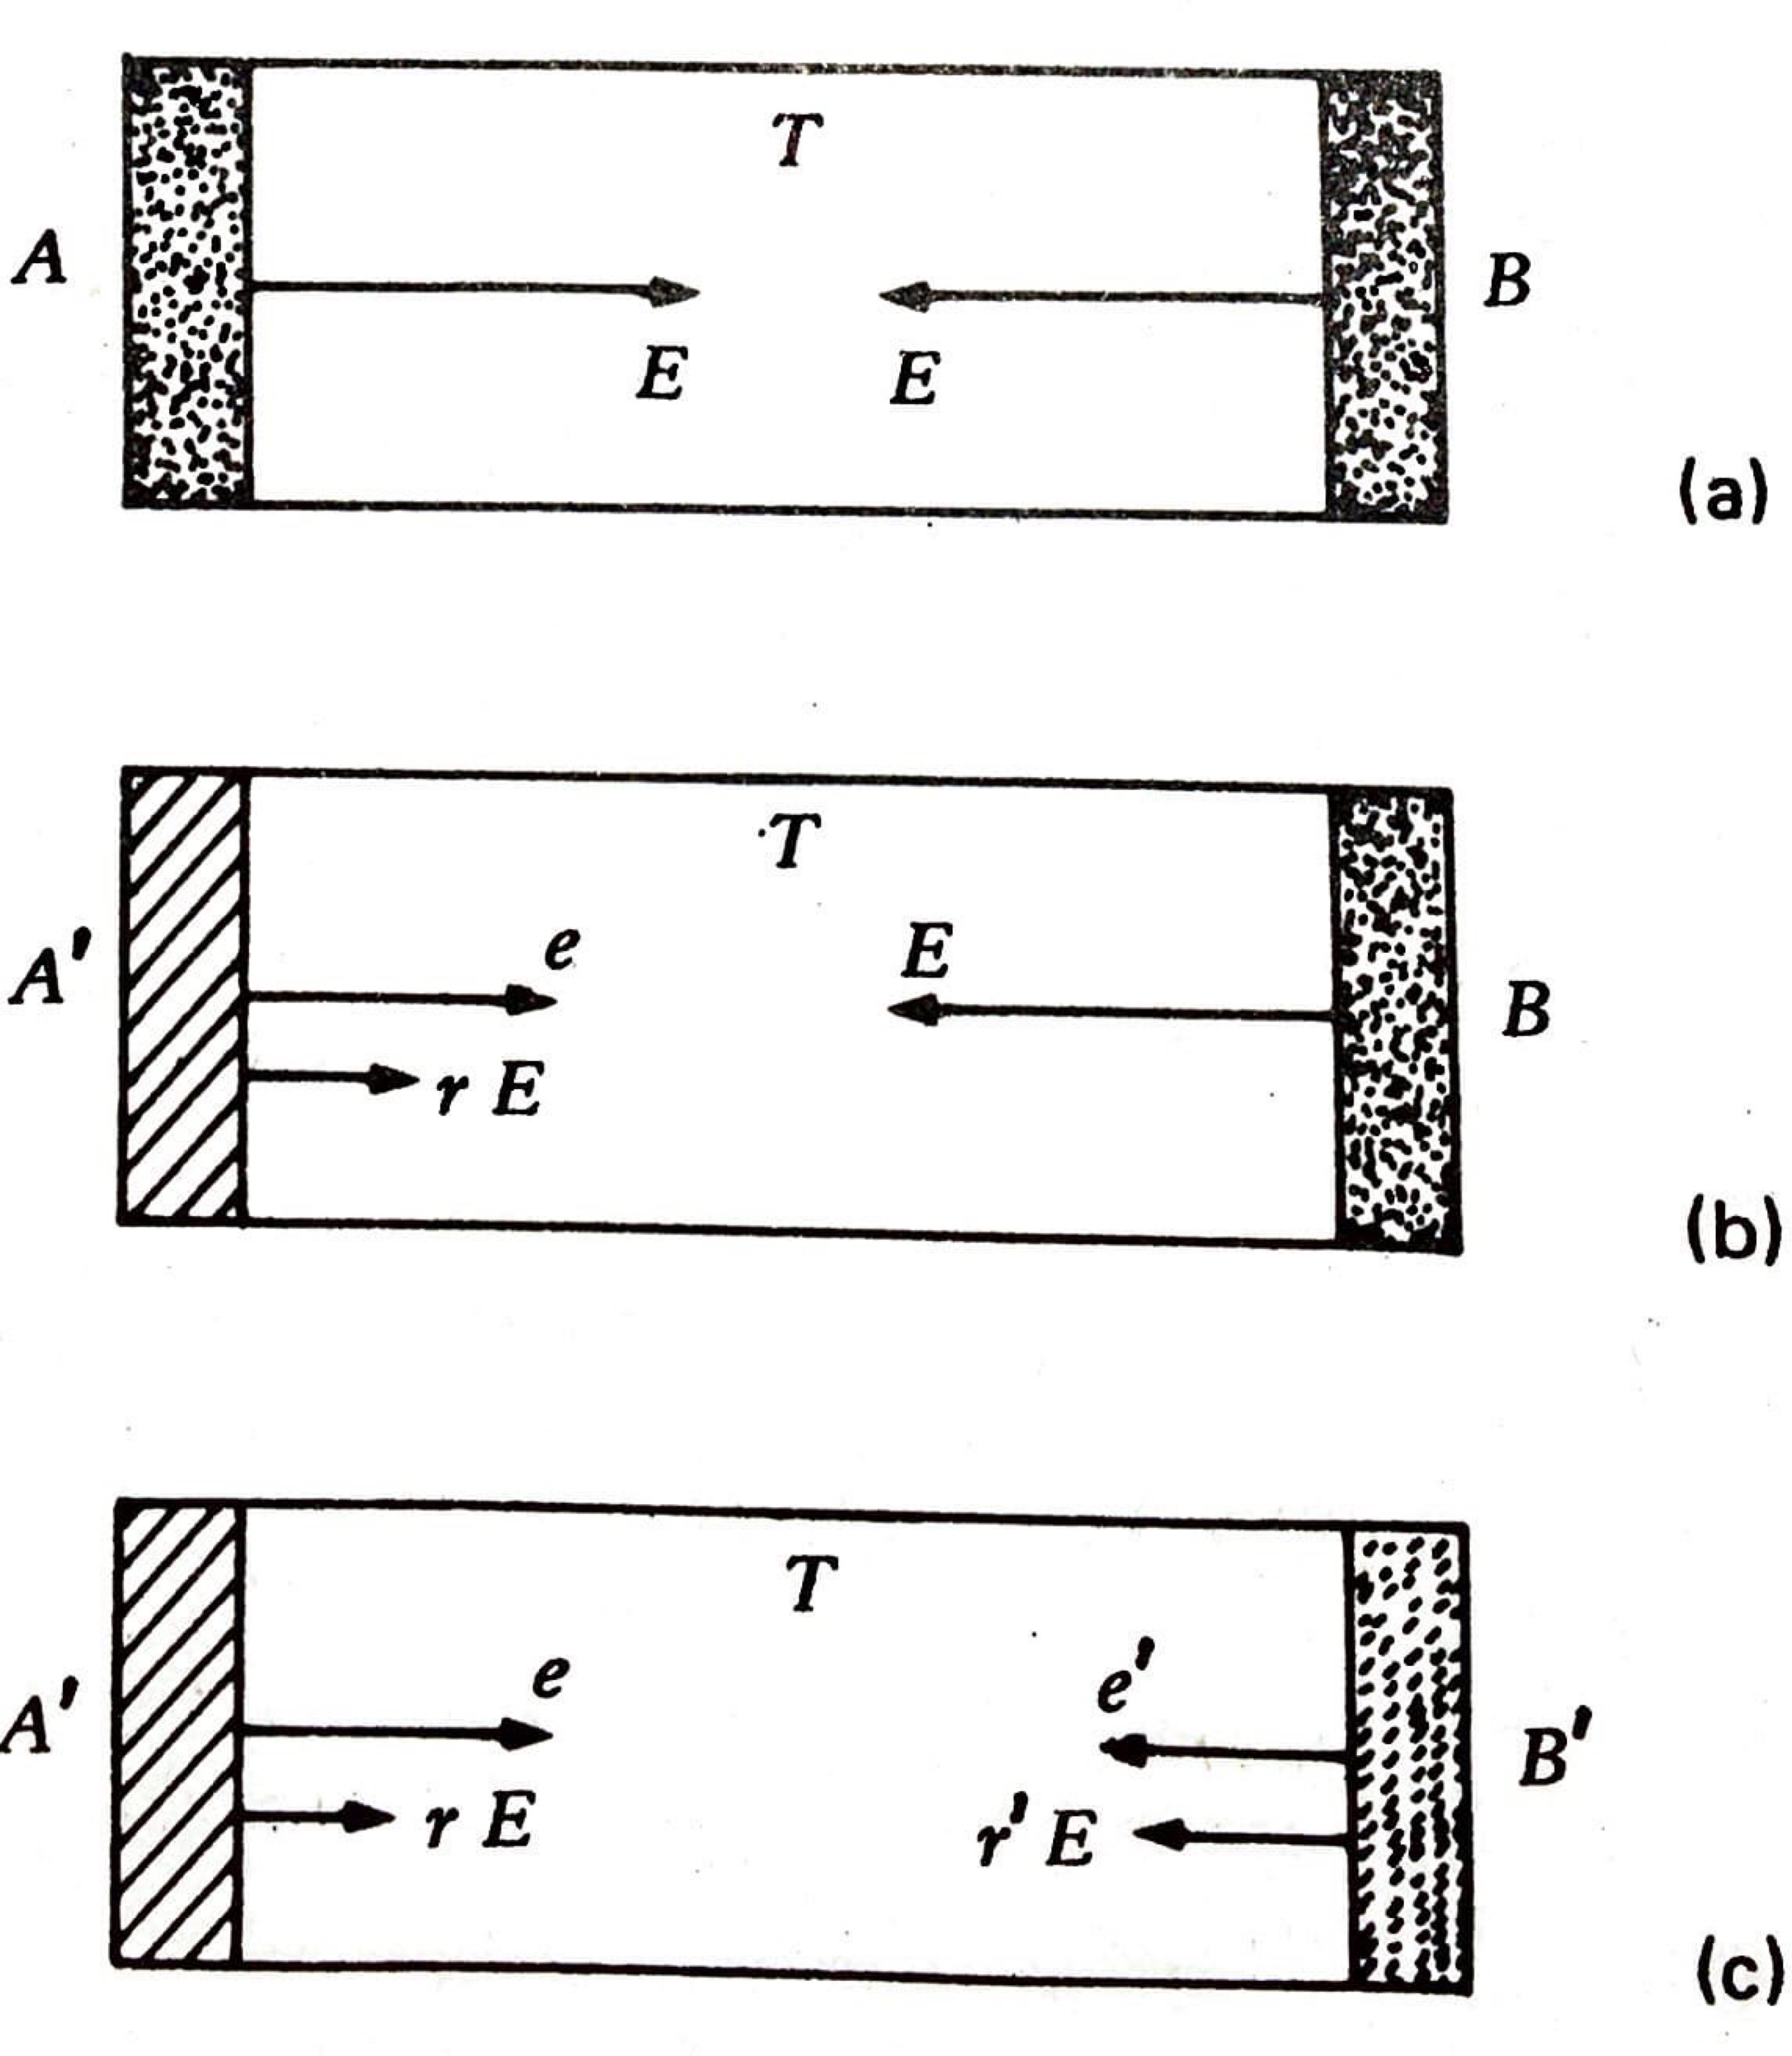
\includegraphics[trim={0cm 0cm 0 0},width=0.9\textwidth]{khhff1}
                            %\captionof{khhff1}{Transfer from R1 to R2 whenK1=1}
                        \end{minipage}
                        Due corpi neri diversi A,B alla stessa temperatura: irraggiamento \'e lo stesso perch\'e se irr. di A fosse maggiore di B la temperatura di B aumenterebbe e diminuirebbe quella di B  - viola secondo principio termodinamica ($\TDy{t}{S}\geq0$: calore ceduto da corpo a temperatura minore negativo assorbito da corpo a temperatura maggiore (+) quindi avremmo diminuzione entropia). In conclusione A e B debìvono irradiare la stessa energia per unit\'a di area.
                        Sostituiamo ad A un corpo non perfettamente nero A' dotato di potere emissivo $e$ ed assorbente $a$, E potere emissivo di B di corpo nero: A' emette $e$ \si{\per\square\cm} ed \'e investito da B di cui assorbe $aE$, perch\'e i due corpi si mantengano alla stessa temperatura occorre che $aE=e$ cio\'e $\frac{e}{a}=E$ che non dipende dalla natura del corpo; d'altra parte A' ha potere riflettente r quindi riflette energia $Er$ e all'equilibrio termico l'energia inviata da A' deve eguagliare quella inviata da B $E=(r+a)E=rE+aE=rE+e$, cio\'e A' e B inviano stessa energia.
                        Sostituiamo B con B' non nero con potere emissivo $e_1$, assorbente $a_1$, riflettente $r_1$: il corpo $A'$ emette energia $e$ e per conservare T deve ricevere da $B'$ l'energia $Ea$, cio\'e l'energia che $A'$ riceve \si{\per\square\cm} non dipende dalla natura di B.
                        Questo vale quando si raggiunge equilibrio termico (equilibrio tra emissione e assorbimento)
                    \item Generalizzazione a qualsiasi $\nu$: supponiamo per assurdo che questa relazione non sia valida per tutti i valori di $\nu$. Sia B nero ma A no alla stessa T: tra essi c'\'e lo stesso scambio di energia totale; supponiamo per assurdo:
                        \begin{align*}
                            e(\nu_1,T,x)d\,\nu>a(\nu_1,T,x)E(\nu_1,T)\\
                            e(\nu_2,T,x)d\,\nu<a(\nu_2,T,x)E(\nu_2,T)%\label{}
                        \end{align*}
                        Supponiamo di dividere il cilindro con una lastra trasparente per l'onda $\nu_1$ e opaca per $\nu_2$ compresa tra due specchi: abbiamo inizialmente due camere distinte nelle quali si stabiliscono radiazioni nere con stessa densit\'a di energia dato che T \'e la stessa ma a sinistra avremo prevalenza di $\nu_1$; togliamo gli specchi: onda $\nu_1$ propaga energia per ristabilire la stessa densit\'a di energia per onda $\nu_1$ ma ci\'o provoca emissione da A e diminuzione di T e aumento di T per B. Assurdo: \ref{pkhhff} \'e valida sempre.
                \end{itemize}
            \section{densit\'a energia radiante in una cavit\'a}
                Una cavit\'a con pareti assorbenti in equilibrio termico si ha radiazione nera; determino relazione tra densit\'a di energia della cavit\'a e potere emissivo. Su unit\'a di superficie arriva nell'unit\'a di tempo e per angolo solido $d\,\Omega$ l'energia contenuta entro una distanza percorsa da c in unit\'a di tempo e la stessa energia viene emessa dalla superficie: densit\'a di energia $d(\nu,T)=\frac{2}{c}E(\nu,T)\int d\,\Omega=\frac{4\pi}{c}E(\nu,T)$; analogamnete per corpo non nero $d(\nu,T)=\frac{4\pi}{c}\frac{e(\nu,T,x)}{a(\nu,T,x)}$, ovvero per pareti in equilibrio termico si ottiene relazione precedente.
        \section{Pressione di Radiazione: esperimento termodinamico}
            \subsection{La radiazione esercita pressione} 
                Ciclo termodinamico - Considero cilindro a  pareti adiabatiche con basi due corpi assorbenti qualunque mantenuti a $B:T_2<T_1:A$ e uno stantuffo riflettente per ora vincolato a $s_1$ in maniera che possa andare solo verso A($T_1>T_2$): la densit\'a di energia $d_1>d_2$; inseriamo stantuffo a $s_2$ vicino B: abbiamo intrappolato della radiazione tra stantuffo 1 e 2 e spostando 2 da $s_2$ la densit\'a aumenta dal valore iniziale $d_2$ fino a raggiunger $d_1$: la parte con densit\'a $d_1$ \'e ora maggiore a scapito dell'energia fornita da B; se continuiamo a spostare stantuffo 2 verso A l'energia in eccesso \'e assorbita da A e quella mancante fornita da B fino a raggiungere $s_1$: tutta l'energia contenuta tra i due stantuffi \'e passata in A e il sistema \'e ritornato alle condizioni iniziali; per secondo principio della termodinamica \'e possibile trasferire calore da corpo a temperatura minore a uno a temperatura maggiore solo facendo lavoro per spostare gli stantuffila radiazione esercita pressione sui corpi su cui incide.
            \subsection{Pressione proporzionale alla densit\'a di energia}i
                Immaginiamo di spingere stantuffo 1 verso  A di un tratto l: sia S la superficie dello stantuffo e $P_1,P_2,d_1,d_2$ la pressione, energia nelle due parti, A assorbe energia $d_1lS$, mentre B emette $d_2lS$ e il lavoro compiuto sullo stantuffo \'e $L=(P_1-P_2)lS$ quindi $(P_1-P_2)lS=(d_1-d_2)lS$ e si vede che $d=P$.
                Infine considerando la media sulle 3 dimensioni si ha $P=\frac{1}{3}d$(parete assorbente). EOS: $PV=\frac{1}{3}dV=\frac{1}{3}U$ (Gas perfettomonoatomica: $PV=NkT=\frac{2}{3}U$).
        \section{Radiation pressure: momentum trasfer(chandra: pg 191)}
            \subsection{Momentum transfer across element surface} 
                    Radiation of energy E traversin medium in a gi ven direction carries momentum $\frac{E}{c}=\frac{h\nu}{c}$ and to calculate radiation pressure at P we need to consider net momentum transfer across arbitrarily element surface $dS$ containing P: radiation energy traversing surface at angle $\theta$ to normal of $dS$ in directions specified by $d\Omega$ in time $dt$ is $I_{\nu}\cos{\theta}d\,\Omega d\,\nu d\,Sd\,t$, hence normal component to $dS$ of momentum is $\frac{1}{c}d\,Sd\,tI_{\nu}\cos^2{\theta}d\,\Omegad\,\nu$; if the radiation is isotropic the integration over sphere reduce to
                    \begin{equation*}
                    P_{RAD}=2\pi I_{\nu}\frac{1}{c}\int_0^{\pi}\cos^2{\theta}\sin{\theta}d\,\theta=\frac{4}{3c}\pi I_{\nu}    
                    \end{equation*}
            \subsection{Energy density of radiation}
                    Let take invi nitesima element volume $v$ centered at P, delimited by surfase $\sigma$(convex); we surround $\sigma$ by much bigger surface $\Sigma$(convex) but suff. small that intensity in a given dir. is the same for all points inside. Energy flowing across $d\,\Sigma$ and $d\,\sigma$ per unit time $I \frac{\cos{\theta}\cos{\Theta}d\,\sigma d\,\Sigma}{r^2}$ where $\theta,\Theta$ are angles made by direction connecting two element surface and their normals; being l distance travelled by light inside v, total amount of radiant energy transiting through $v$ by considered pencil is:
                    \begin{align*}
                    &I \frac{\cos{\theta}\cos{\Theta}d\,\sigma d\,\Sigma}{r^2}\frac{l}{c}\\
                    &=I \frac{d\,v}{c}d\,\omega\\
                    &d\,v=l\cos{\theta}d\,\sigma\\
                    &d\,\omega=\frac{\cos{\Theta}d\,\Sigma}{r^2}&\tag{solid angle}
                    &&\tag{subtended by $d\,\Sigma$ at P}
                    \end{align*}
                    and total energy transiting through v from all dir. is $\frac{1}{c}\int\int Id\,vd\,\omega=\frac{v}{c}\int Id\,\omega$ and density
                    \begin{equation}
                        u=\frac{1}{c}\int Id\,\omega
                    \end{equation}
                    For isotropic radiation $u=\frac{4\pi}{c}I$
            \subsection{Relation between energy density and radiation pressure}
            \subsection{Mechanical force exerted by radiation}
                Thin cylinder of crosssection $d\,\sigm$ and length $ds$ in the dir. normal to $d\,\sigma$; amount radiant energy incident on $d\,\sigma$ in direction of solid angle $d\,\omega$ about dir. at angle $\theta$ with s-dir is $I_{\nu}\cos{\theta}d\,\sigma d\,\omega d\,\nu$ and the amount of energy absorbed by cylinder is $I_{\nu}\cos{\theta} d\,\sigma d\,\omega d\,\nu\kappa_{\nu}\rho\sec{\theta}d\,s$, ($\sec{\theta}=\frac{1}{\cos{\theta}}$), $\sec{\theta}d\,s$ is length of path intercepted in cylinder by pencil, and divided by c is the amount of momentum comunicated in direction of $I_{\nu}$ so the normal component (to $d\,\sigma$) is: 
                \begin{equation*}
                    I_{\nu}\cos{\theta}d\,\sigma d\,\omega d\,\nu\kappa_{\nu}\rho\sec{\theta}d\,s \frac{1}{c}\cos{\theta}
                \end{equation*}
                dividing by surface $d\sigma$ and integrating over all dirs of incident rad. we obtain for force per unit area of a cyl slab of thickness $ds$:
                \begin{equation*}
                    \frac{\kappa_{\nu}\rho d\,s}{c}\int I_{\nu}\cos{\theta}d\,\omega d\,\nu
                \end{equation*}
                Spontaneous emission is uniform in all dir so no net force. Induced emission is in pencil direction so it's opposite to absorption.
        \section{Termodinamica radiazione nera: Legge di Stefan-Boltzmann}
                Il calore irraggiato dal corpo nero \'e $E(T)=\sigma T^4$.
                Macchina di Carnot reversibile che lavara su radiazione nera: considero cilindro di volume V adiabatico chiuso da stantuffo contenente radiazione di corpo nero a temperatura T. Per PTII:
                \begin{align*}
                    &\PDy{V}{U}|_T=T\PDy{T}{P}|_V-P,\ U(V,T)=Vd(T):\\
                    &d(T)=T\PDy{T}{P}|_V-P,\ P=\frac{1}{3}d:\\
                    &4\frac{d(T)}{T}=\PDy{T}{d(T)}\Rightarrow d(T)=\const{}T^4
                \end{align*}
                E ricordando la relazione tra potere radiante E(v. P di \khhff) e la densit\'a di energia radiante si ha la legge si SB $E(T)=\sigma(T^4-T_0^4)$.
                \section{Legge di Wien}
                Wien immagina di racchiudere l'energia emessa da corpo nero in uno dei soliti cilindri con stantuffo mobile: se lo stantuffo si sposta comprimendo energia tale densit\'a va aumentando e cresce per tutte $\lambda$ ma a causa Doppler lunghezza riflessa durante spostamento \'e pi\'u piccola.
                \begin{itemize}
                    \item Il potere emissivo:
                        \begin{align*}
                            &E(\lambda,T)=T^5f_1(\lambda T)\\
                            &E(\lambda,T)d\,\lambda=T^5f_1(\lambda T)d\,\lambda=\lambda\invers{5}(\lambda T)^5f_1(\lambda T)d\,\lambda=\lambda\invers{5}f_2(\lambda T)\Tdy{\nu}{\lambda}d\,\lambda=-\frac{\nu^5}{c^5}f_2(\cfrac{T}{\nu})\frac{c}{\nu^2}d\,\nu\tag{$\lambda=\frac{c}{\nu}$}\\
                            &=\nu^3f(\frac{\nu}{T})d\,\nu
                        \end{align*}
                \end{itemize}
\part{Ripeto EM}

\part{Ripeto scattering}

\part{Ripeto statistical physics}

\part{Ripeto QM-Atomo d'idrogeno}

\part{Principio di Kirchhoff}
     \khhff{} ha dimostrato per via termodinamica nel 1860 che per un corpo in equilibrio termodinamico
%\end{document}
%subfile
%\stopcontents[chapters]
\end{document}
